
\section{Evaluation}
\label{sec:evaluation}
We deployed our system over nine geo-distributed datacenters of Amazon EC2 and evaluated with a synthetic workload and two realistic applications, namely TPC-C and RUBiS. The evaluation includes two variations of our STR, one that only performs speculative read ({\specula}-Internal) and one that can perform both speculative read and speculative commit ({\specula}-External), against two transactional protocols. The results show that even without externalizing speculative results, we can achieve about 3.5$\times$ speedup for workloads with high local contention and low remote contention. Nevertheless, allowing speculative commit can further reduce latency by XXX. \textbf{How to write latency reduction? For some workload, our final latency is 300 while the baselin is 21000, so we say by a factor or 70? What about for perceived latency?}

\subsection{\specula variations and baselines}
We implemented two variations of \specula, namely {\specula}-Internal and  {\specula}-External. {\specula}-Internal only allows speculative read, which means it does not externalize speculative results (with respect to 'internal') and does not require writing compensation logic; on the other hand, {\specula}-External allows both speculative read and speculative commit, which may externalize speculative results. Both protocols are run with an automatic tuning process. The automatic tuning process collects throughput statistics from all servers every twenty seconds \textbf{should I mention that?}, then it calculates the next speculation level and informs all servers. The tuning starts with the most conservative speculation level, i.e. no speculative read and no speculative commit, then proceeds until it finds a speculation level that gives the maximal throughput. The possible speculation levels, from conservative to aggressive, are: no speculative read (No SR), only speculative read (SR, the maximal level {\specula}-Internal can have), speculative read and speculative commit with length one (SR+SL1), ..., till SR+SL8 (the maximal level {\specula}-External can have).

We built two baseline protocols for comparison. The first one is based on ClockSI \cite{clocksi}, a decentralized transactional protocol that provides Snapshot Isolation. The original ClockSI protocol does not support replication and we added a simple replication mechanism: when a master partition receives a prepare request, it synchronously replicates it to its replicas. Then replicas  acknowledge the transaction coordinator directly and the coordinator commits the transaction when it has received prepare from all involved partitions and their replicas. The protocol requires one and half WAN round-trip to commit a transaction. We name it as ClockSI-Rep. We also built a baseline protocol that intends to emulate PLANET \cite{pang2014planet}, which permits speculatively committing transaction while not allowing speculative read or pipelining speculative transactions. As in the original paper, PLANET is built on top of the MDCC protocol \cite{kraska2013mdcc} and uses a prediction model to decide whether to speculate. Since it is not possible to do an apple-to-apple comparison, we implemented a simplified version of PLANET, by building it atop ClockSI-Rep and additionally allows each client to speculatively commit one transaction. 

\subsection{Experimental setup}
\label{subsec:setup}
We implemented our baseline protocol and \specula using the Erlang programming language, based on \textit{antidote}, an open-source reference platform for evaluating distributed consistency protocols \cite{antidote}.

The system is deployed in nine datacenters of Amazon EC2: Ireland(IE), Seoul(SU), Sydney(SY), Oregon(OR), Singapore(SG), North California(CA), Frankfurt(FR), \\ Tokyo(TY) and North Virginia(VA). Each datacenter consists of three m4.large instances (2 VCPU and 8 GB of memory) and each instance holds the master replica of one partition. All DCs form a consistent hashing ring according to the order in the above list; the data of each instance is replicated by five following datacenters' corresponding servers, e.g. the data of DC CA is replicated by DCs FR, TY, VA, IE and SU. We interleave DCs from nearby regions in the hash ring, so that different replication group will have similar latency to perform replication, as shown in table \ref{tab:latency}.

A workload stressor is located in each instance. It spawns some number of threads (clients) to issue transactions to local transaction coordinators and retries a transaction if it gets aborted. The final latency of a transaction is calculated as the duration from its first trial to its commit time, and the user perceived latency (for speculative commit) is measured as the duration from its first trial to its last speculative commit (after which it commits). Last but not least, each experiment is run for three times. We discard the aggregate results of the first twenty seconds and show the average value (deviation is low).

\begin{table*}
\small
\begin{center}
  \begin{tabular}{l |  l | l | l| l | l | l| l| l |l } 
     & IE & SU& SY& OR & SG & CA &  FR & TY & VA  \\ \hline
  \textbf{Max latency (replicas)} & 334(SG) & 267(FR) & 321(FR) & 160(SG)  & 337(IE) & 167(FR) & 321(SY)& 212(IE)  &  226(SY)  \\   \hline
  \textbf{Max latency (all)} &  334(SG) &  267(FR) & 321(FR)  & 163(SY) & 337(IE) & 175(SG) & 324(SG)  & 233(FR)  & 226(SY) \\ \hline
  \end{tabular}
\end{center}
\caption{Maximal mean latency of a DC to its replicas and to all other DC}
\label{tab:latency}
\end{table*}

\subsection{Synthetic workloads}
Our evaluation starts with synthetic workloads. The synthetic workloads represent idealistic non-interactive workloads, where each thread issues a new transaction as soon as the previous one is committed (or speculative committed). In these experiments, we pick four representative contention levels to check the performance of these protocols.

\paragraph{Transaction and data access} A transaction reads 10 keys then updates them. When accessing a data partition, 90\% of key access goes to a small range of that data partition, a.k.a hotspot, and we adjust the size of hotspot to control contention rate. Each data partition has two million keys, of which one million are only accessible by local-initiated transactions and the other are only accessible by remote transactions. This allows adjusting local contention level (i.e. the contention that happens when a transaction performs local certification) without affecting remote contention level. In the following experiments, we denote 30000 keys for the size of local hotspot size as low local contention and 1000 keys as high local contention; according, 15000 keys for a remote hotspot is named low remote contention and 500 keys for high remote contention. 80\% of a transaction's key access goes to local master partitions, while 20\% goes to slave data partitions replicated locally.

\begin{figure*}
\centering
\def\svgwidth{0.98\columnwidth}
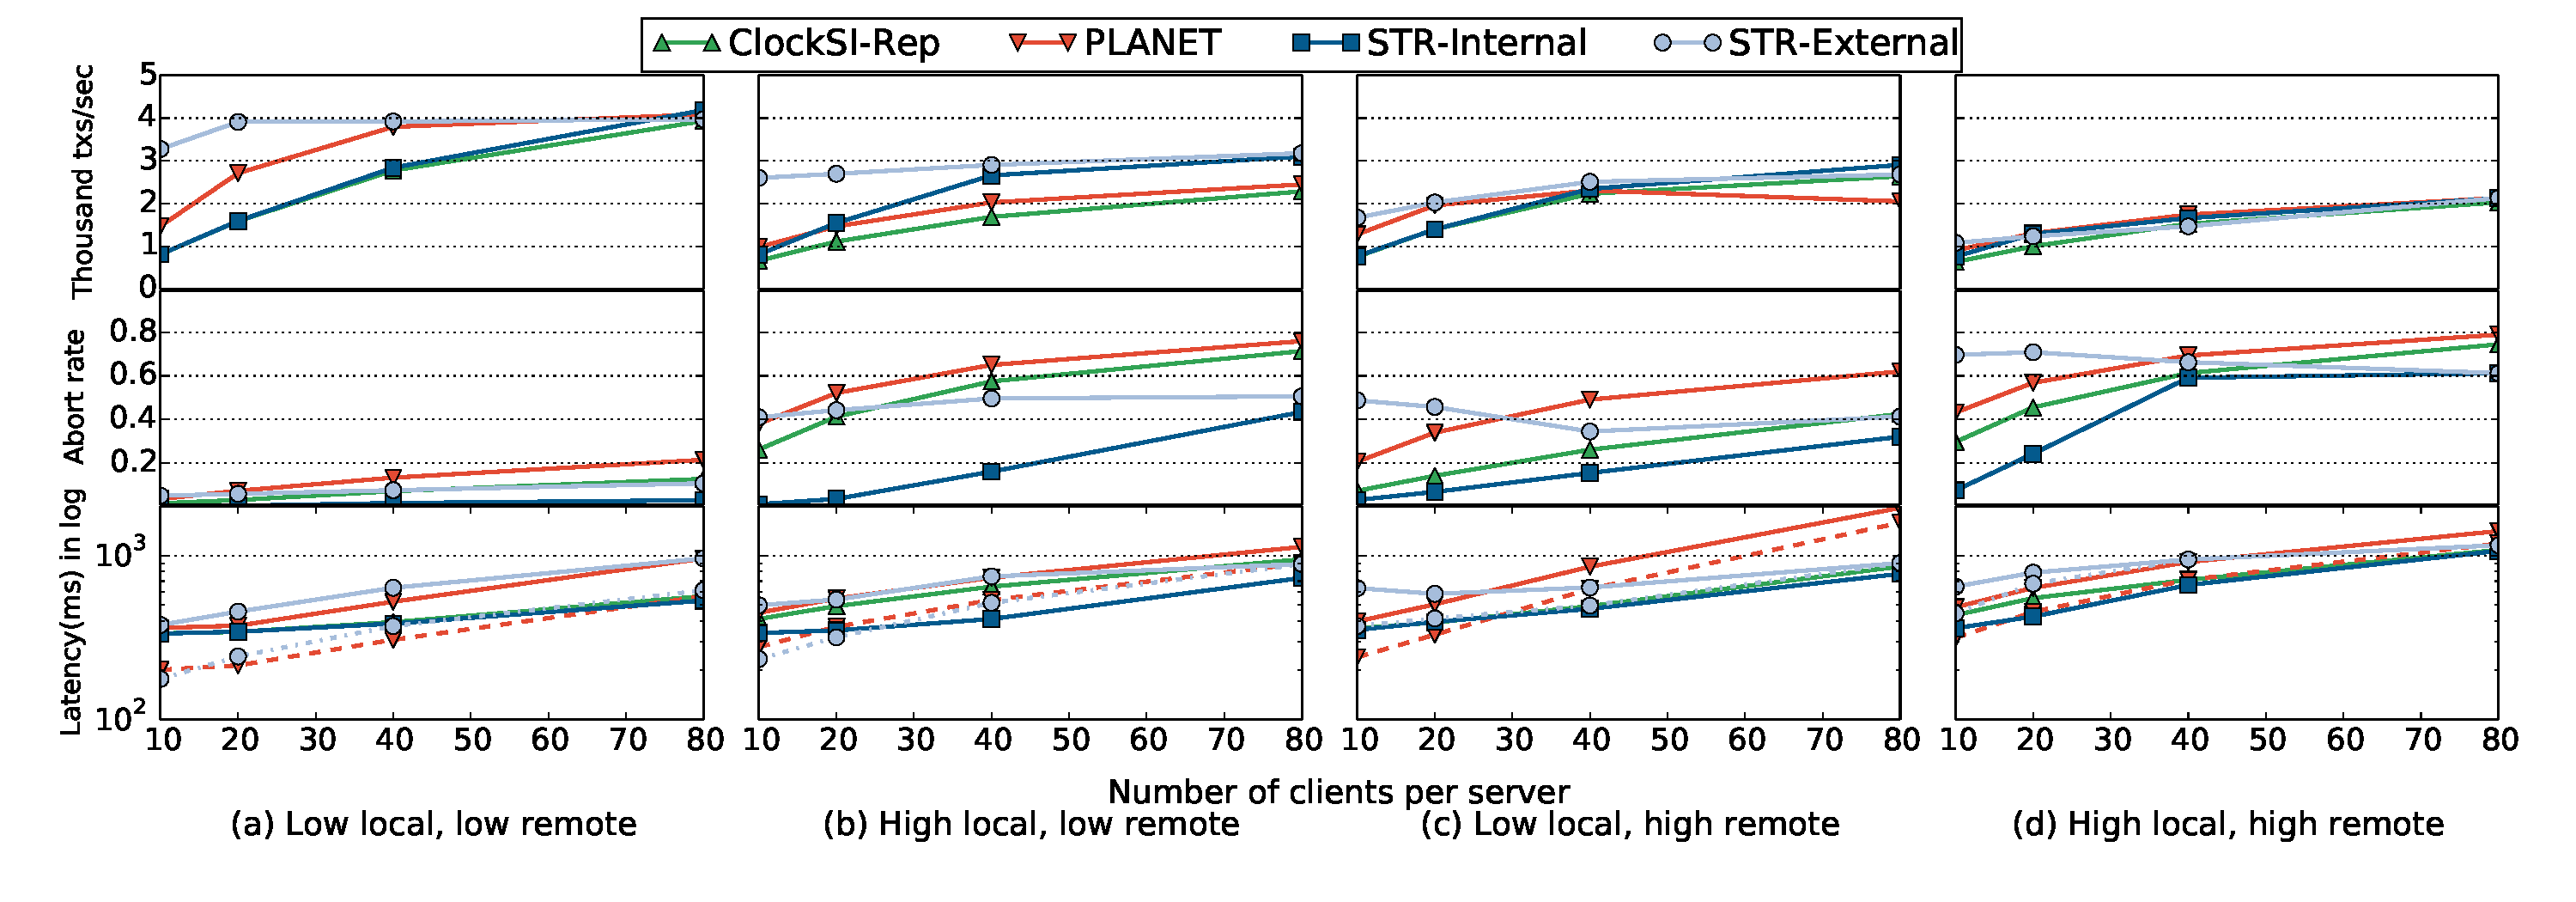
\includegraphics[scale=0.35]{figures/micro}
\vspace{-9mm}
\caption{\small \textit{Performance of different protocols under four levels of contention.} \textit{Low local, low remote} denotes low local contention and low remote contention, and so forth. For latency, solid lines denote a transaction's final latency and dashed lines denote a transaction's perceived latency.}
\label{fig:micro}
\end{figure*}


\begin{figure}[t]
\centering
\def\svgwidth{0.98\columnwidth}
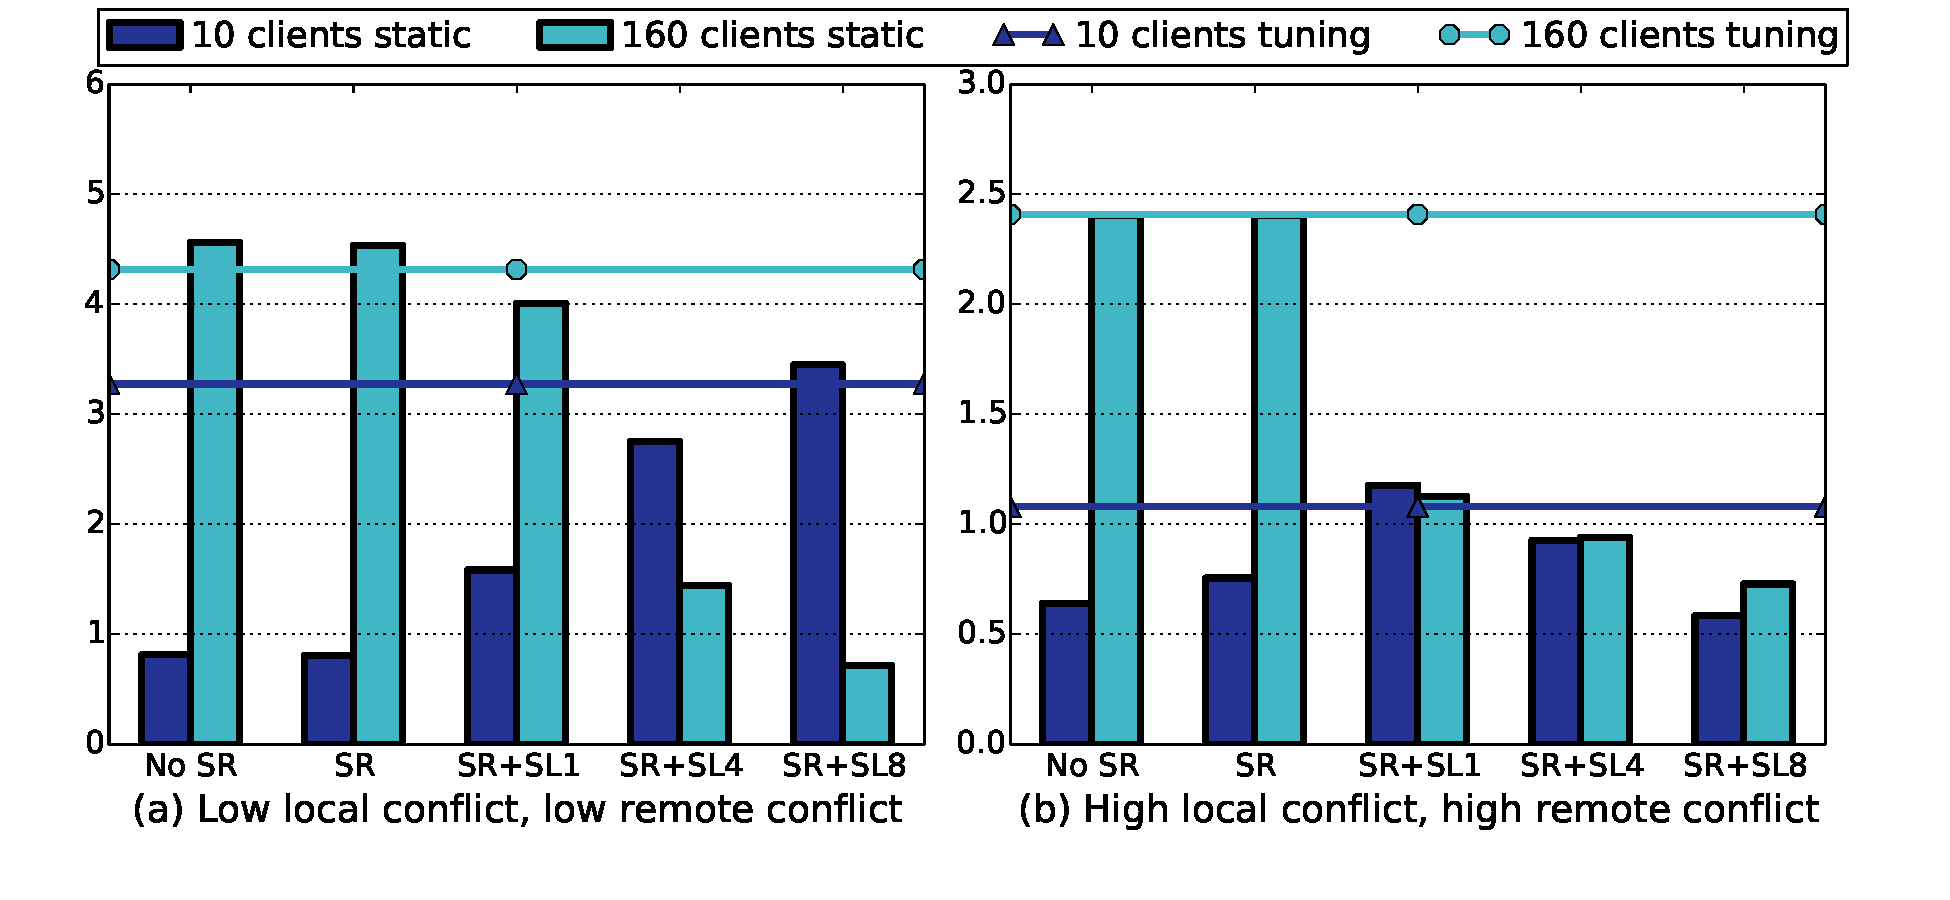
\includegraphics[scale = 0.28]{figures/tuning}
\vspace{-9mm}
\caption{\small The throughput of tuning versus static configuration}
\label{fig:tuning}
\end{figure}

\paragraph{Performance under different contentions} First, we examine a workload with both low local contention and low remote contention. As shown in figure \ref{fig:micro}a, both PLANET and {\specula}-External achieve good speedup compared with the baseline, because they all allow speculatively committing transactions so clients can perform more optimistic work during transaction certification. Since {\specula}-External can pipeline multiple speculative transactions, it almost achieves the peak throughput (4K txs/sec) with 20 clients, while PLANET needs about 40 clients. The figure also presents the final latency with solid lines and perceived latency (for {\specula}-External and PLANET) with dashed lines. {\specula}-External and PLANET provide low perceived latency at low load, but latency grows with larger number of clients because they allow speculative commit, which are more likely to fail and cause retry when contention increases (due to more number of clients). {\specula}-Internal has little performance gain over ClockSI-Rep, as there is low contention so it has little chance to performance speculative read, but its abort rate is still lower than ClockSI-Rep due to the use of PreciseClock. 

Figure \ref{fig:micro}b shows a workload with high local contention and low remote contention. This is a favorable workload for {\specula}-Internal and {\specula}-External that allows speculative read, as they can avoid getting blocked when trying to read pre-commit records, and transactions being speculatively-read are likely to commit due to low remote contention. With 80 clients, both {\specula}-Internal and {\specula}-External achieve about a throughput of about 3K transactions per second, 120\% to the peak throughput of ClockSI-Rep. On the other hand, PLANET achieves little performance gain as transactions often gets blocked during execution and have little chance to speculative commit. The effect of speculative read is directly reflected in latency: when there is low load, the latency of PLANET and ClockSI-Rep considerably increase compared with figure \ref{fig:tuning}a, while the latency of {\specula}-Internal and {\specula}-External are not affected due to speculative read.

Next, we examine workloads with high remote contention, which is unfavorable for speculation. As figure \ref{fig:micro}c shows, PLANET has large performance penalty and large latency, as speculative commit often fails due to high remote contention. Although {\specula}-Strong also allows speculative commit, thanks to the automatic tuning method, it can adjust its speculation length to attain near-optimal throughput, despite the contention rate. The performance of STR-Internal are similar to ClockSI-Rep again (as in figure \ref{fig:micro}), due to having low local contention. The last workload combines both high local contention and high remote contention, but {\specula}-External and {\specula}-Internal still remain stable throughput due to auto-tuning. Nevertheless, PLANET has better throughput than in figure \ref{fig:micro}c because high local contention causes transactions to be blocked and perform less speculative commit (which is harmful in this workload).


\begin{figure*}
\centering
\begin{minipage}{.72\textwidth}
\centering
  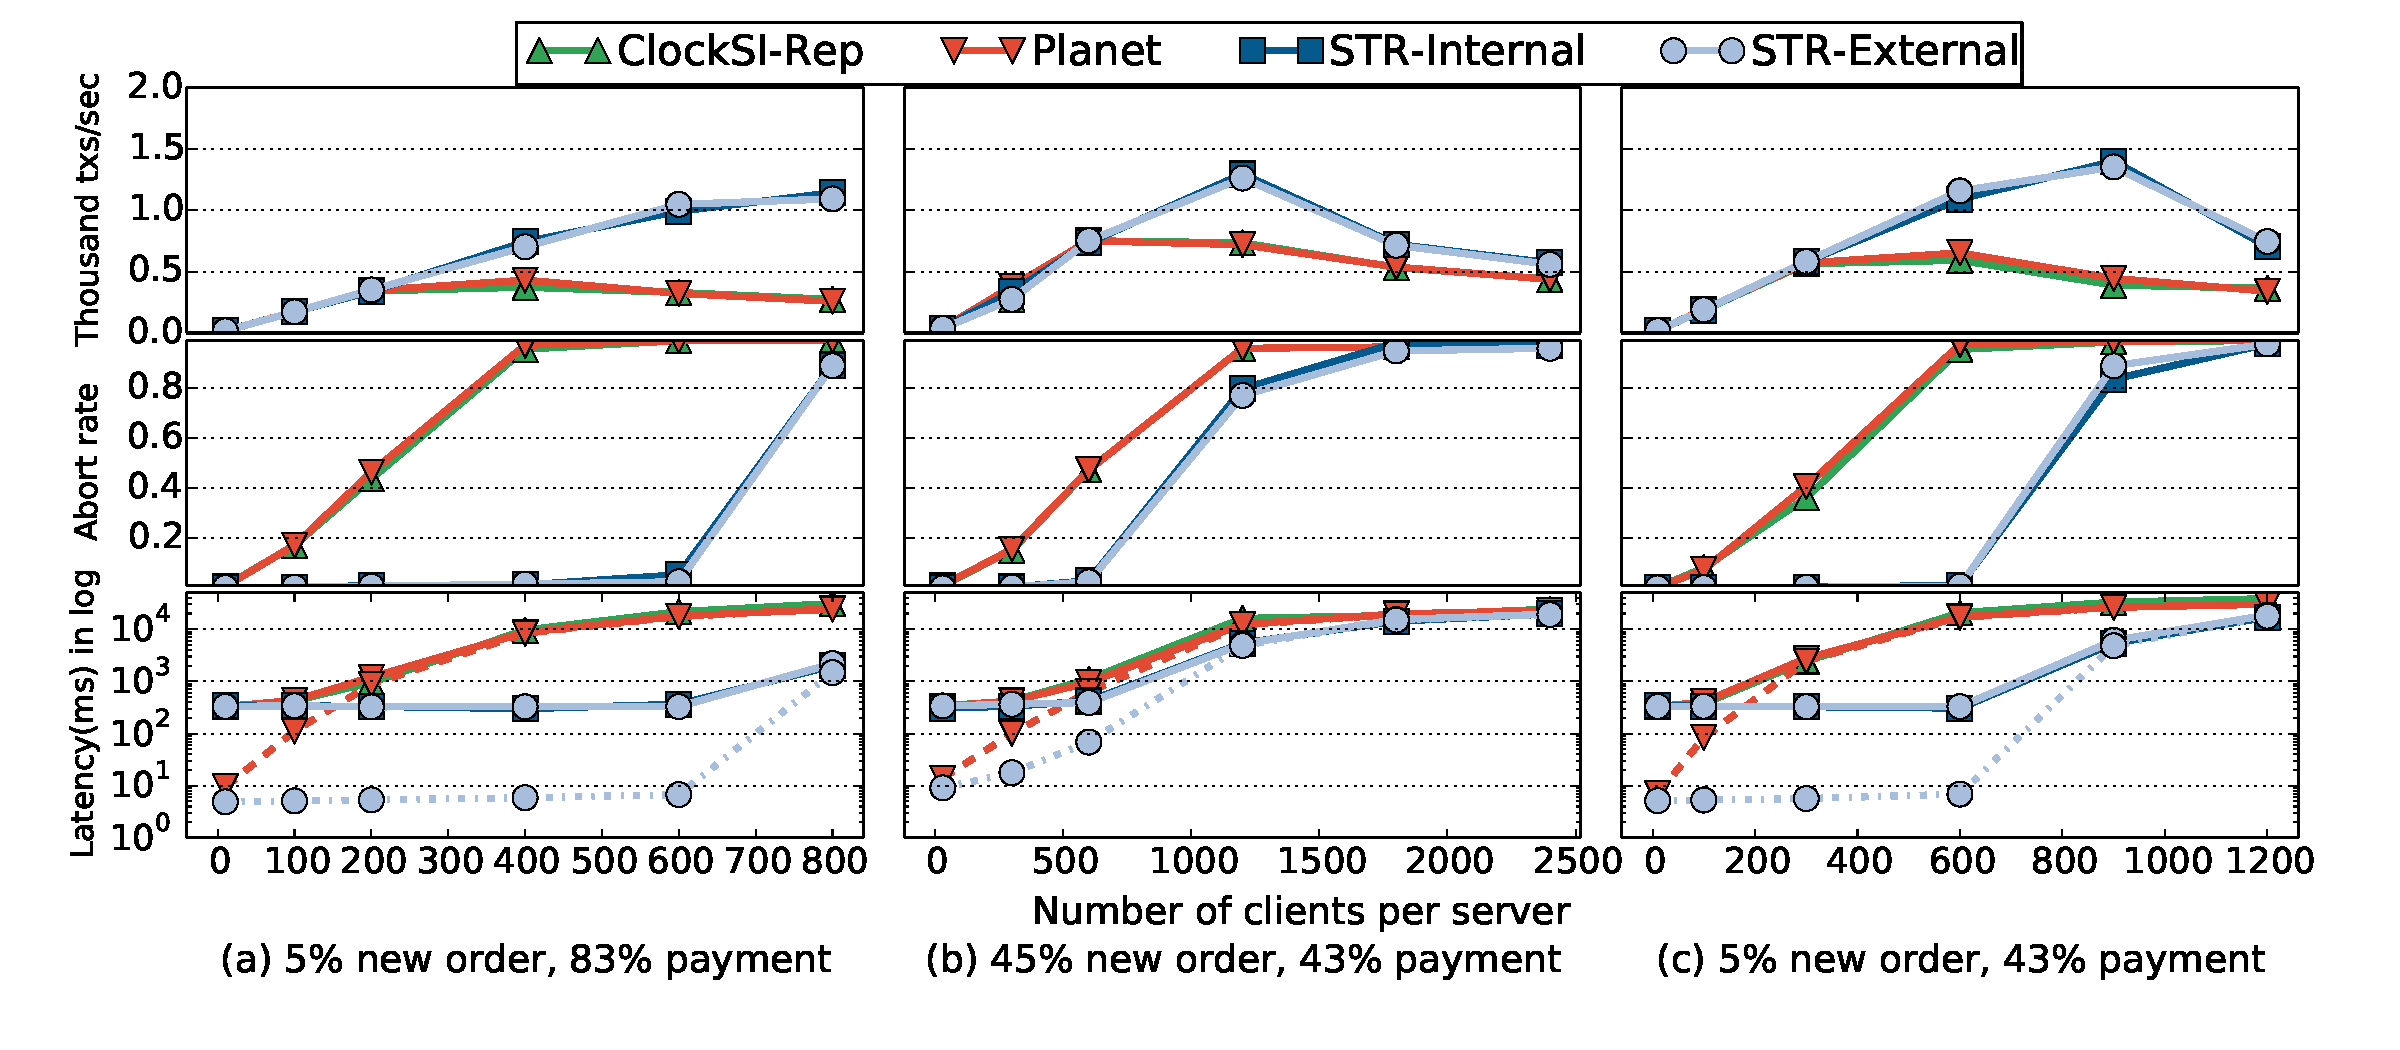
\includegraphics[scale=0.3]{figures/tpcc}
  \vspace{-5mm}
  \caption{\small The performance of different protocols for three TPC-C workloads.}
  \label{fig:tpcc}
\end{minipage}
\begin{minipage}{.26\textwidth}
\centering
  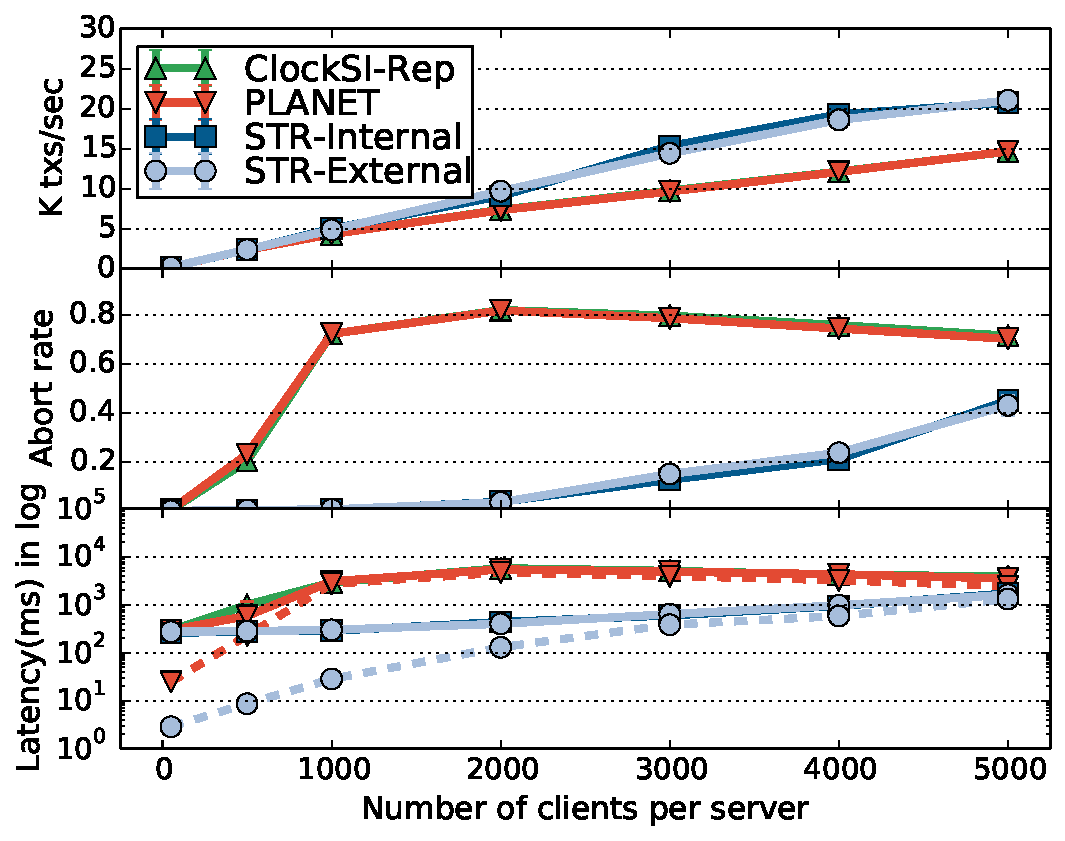
\includegraphics[scale=0.28]{figures/rubislatencywarehouse}
  \vspace{-2mm}
  \caption{\small The performance of different protocols for RUBiS}
  \label{fig:rubis}
\end{minipage}
\end{figure*}


\paragraph{Automatic tuning v.s. static configurations} The previous discussion has shown that the automatic tuning method generally can achieve optimal throughput. However, a hidden fact is that a static configuration of speculation level can have very different performance under different load and different contention. Figure \ref{fig:tuning} compares the throughput of 10 clients and 160 clients per server, using either automatic tuning or different static configuration. We picked two extreme workloads, one with low local and remote contention, and one with high contention for both. The figure shows that the optimal speculation level for throughput varies for contention and load, which is hard to predict in advance. This motivated us to design the automatic tuning method. More importantly, as can be seen in the figure, the curve of speculation level to throughput is convex, i.e. if a speculation level gives local maximal throughput, this is guaranteed to be a global maximum throughput. This observation drove the design of the automatic tuning method to be a simple hill climbing algorithm \cite{hillclimbing}: it starts from no speculative read, then proceeds until it finds a local maximal throughput. Despite being simple and fast, this method can reach throughput close to the optimal throughput.



%Reading a key that is not replicated locally causes large latency, which makes it difficult to examine the benefit of speculation. So for most of the experiments, a transaction only accesses keys replicated in local datacenter. We dedicate a separate experiment to examine the effect of remote read on throughput.

\subsection{Macro benchmark}
In the following experiments, we evaluate the performance of \specula with realistic interactive applications, namely TPC-C\cite{tpcc} and RUBiS \cite{rubis}. The key differences between these workloads and the synthetic ones are: (i) while some synthetic workloads already gives severe contention, some transactions of these two applications, e.g. \textit{payment} of TPC-C and \textit{register\_item} of RUBiS, have even more radical contention, which gives \specula better speedup; (ii) to model realistic human to machine interaction, TPC-C and RUBiS specify large ``think time'' between consecutive operations issued by a user, typically a few seconds, which causes speculative commit to not bring obvious performance improvement. Though, speculative commit can still provides low perceived latency.

\subsubsection{TPC-C}
TPC-C \cite{tpcc} models the workload of an online shopping system. We implemented three TPC-C transactions, namely payment, new-order and order-status, according to the specification. Payment transaction has very high local contention and low remote contention; new-order transaction has medium level local and remote contention, and order-status is a read-only transaction. According to the described workload mix rule in the specification, we use three workloads: 5\% new-order, 83\% payment and 12\% order-status (TPC-C A); 5\% new-order, 43\% payment and 52\% order-status (TPC-C B) and 45\% new-order, 43\% payment and 12\% order-status (TPC-C C). We add the ``think time'' and ``key time'' for each transaction as described in the specification, so a client sleeps for some time (from 5 seconds to as large as hundreds of seconds) both before and after issuing a transaction. A server is loaded with five warehouses (more warehouse means less contention), which reaches the server's memory limit.

As we can see in figure \ref{fig:tpcc}, due to having large think time, speculative commit hardly brings any throughput benefit, while speculative read is beneficial due to these workloads all have high local contention. As a result, PLANET achieves the same throughput as ClockSI-Rep, {\specula}-External achieves the same throughput as {\specula}-Internal, and there is a clear throughput difference between STR and the baselines. Though, with low number of clients, PLANET reduces the perceived latency from about 320 millisecond of ClockSI-Rep to about 10 millisecond, by a factor of 32. But when the load increases, the latency of PLANET also increases as local contention is exacerbated. On the other hand, due to allowing speculative read, {\specula}-External and {\specula-Internal} achieve significant speedup compared with the baseline: 2.93$\times$ for TPC-C A, 1.68$\times$ for TPC-C B and 3.47$\times$ for TPC-C C. Both {\specula} protocols also greatly reduce the operation latency by a factor of about 70 compared with the latency of PLANET and ClockSI-Rep.

\subsection{RUBiS}
RUBiS \cite{rubis} models an online bidding system. Of all the 26 user interactions, there are five update transactions: store bid, store buy now, store comment, register item and register user. RUBiS is designed to run on top of a SQL database, so we did the following modification to adapt it to our key-value store: (i) we horizontally partition database tables across servers, so that each server contains an equal portion of data of each table; (ii) many RUBiS insertion operations need to increment a table index to get unique id, which is inefficient when the table is sharded across machines. To avoid this, we let these operations to update local indices that are maintained by local table shards, as studied in \cite{cecchet2008middleware}. We use RUBiS's 15\% update default workload and its default think time (different transactions can have think time from 2 seconds to 10 seconds).

Due to memory limit, we were not able to load the system with more clients. It is hard to saturate servers with TPC-C workloads, because the default workload is dominated by fast read-only transactions and the contention is lower than TPC-C. Nevertheless, the figure \ref{fig:rubis} still shows that \specula achieves good speedup and latency reduction. With 5000 clients, \specula still achieves about 1.43$\times$ speedup compared with ClockSI-Rep and PLANET. Note that the abort rate of PLANET and ClockSI-Rep slightly decreases with increasing number of clients. This is because in RUBiS, the access pattern of a client highly depends on the update of other clients, so with more number of clients, the access pattern gets more diverse and the abort rate is reduced.

